% !TEX root = msc_thesis.tex

\begin{figure}[tb]
	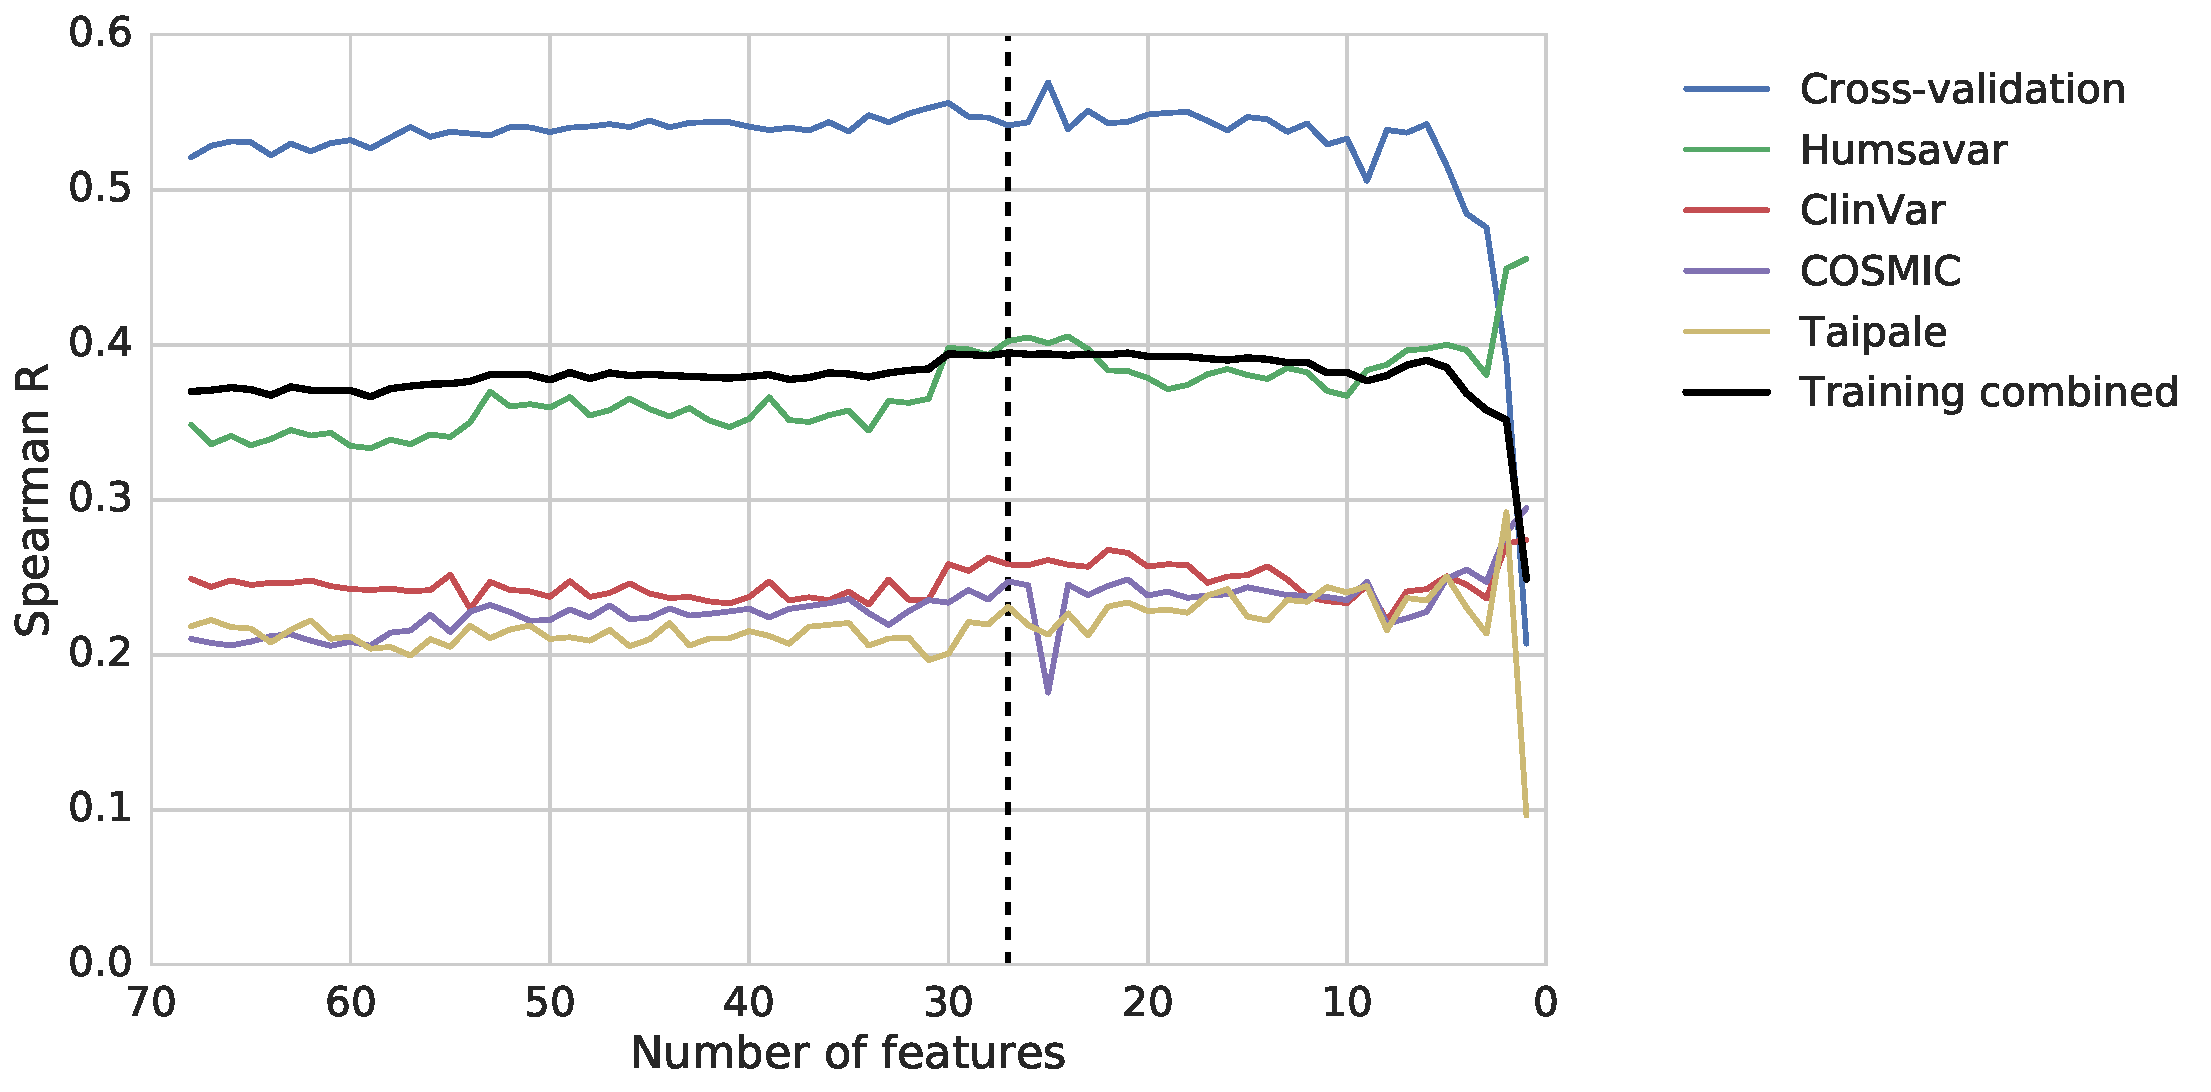
\includegraphics[width=0.9\linewidth]{static/elaspic_training_set/machine_learning/feature_elimination_core.pdf}
	\caption[Core predictor feature elimination.]{
		Performance of the core predictor at each step of feature elimination.
		The combined score (black line) was calculated using Equation \ref{eq:combined_score_core}.
		Predictor with the highest combined score is indicated by the vertical dashed line,
		and the features used to train that predictor are listed in Table \ref{tab:core_features}.
	}
	\label{fig:feature_elimination_core}
\end{figure}

\begin{figure}[tb]
	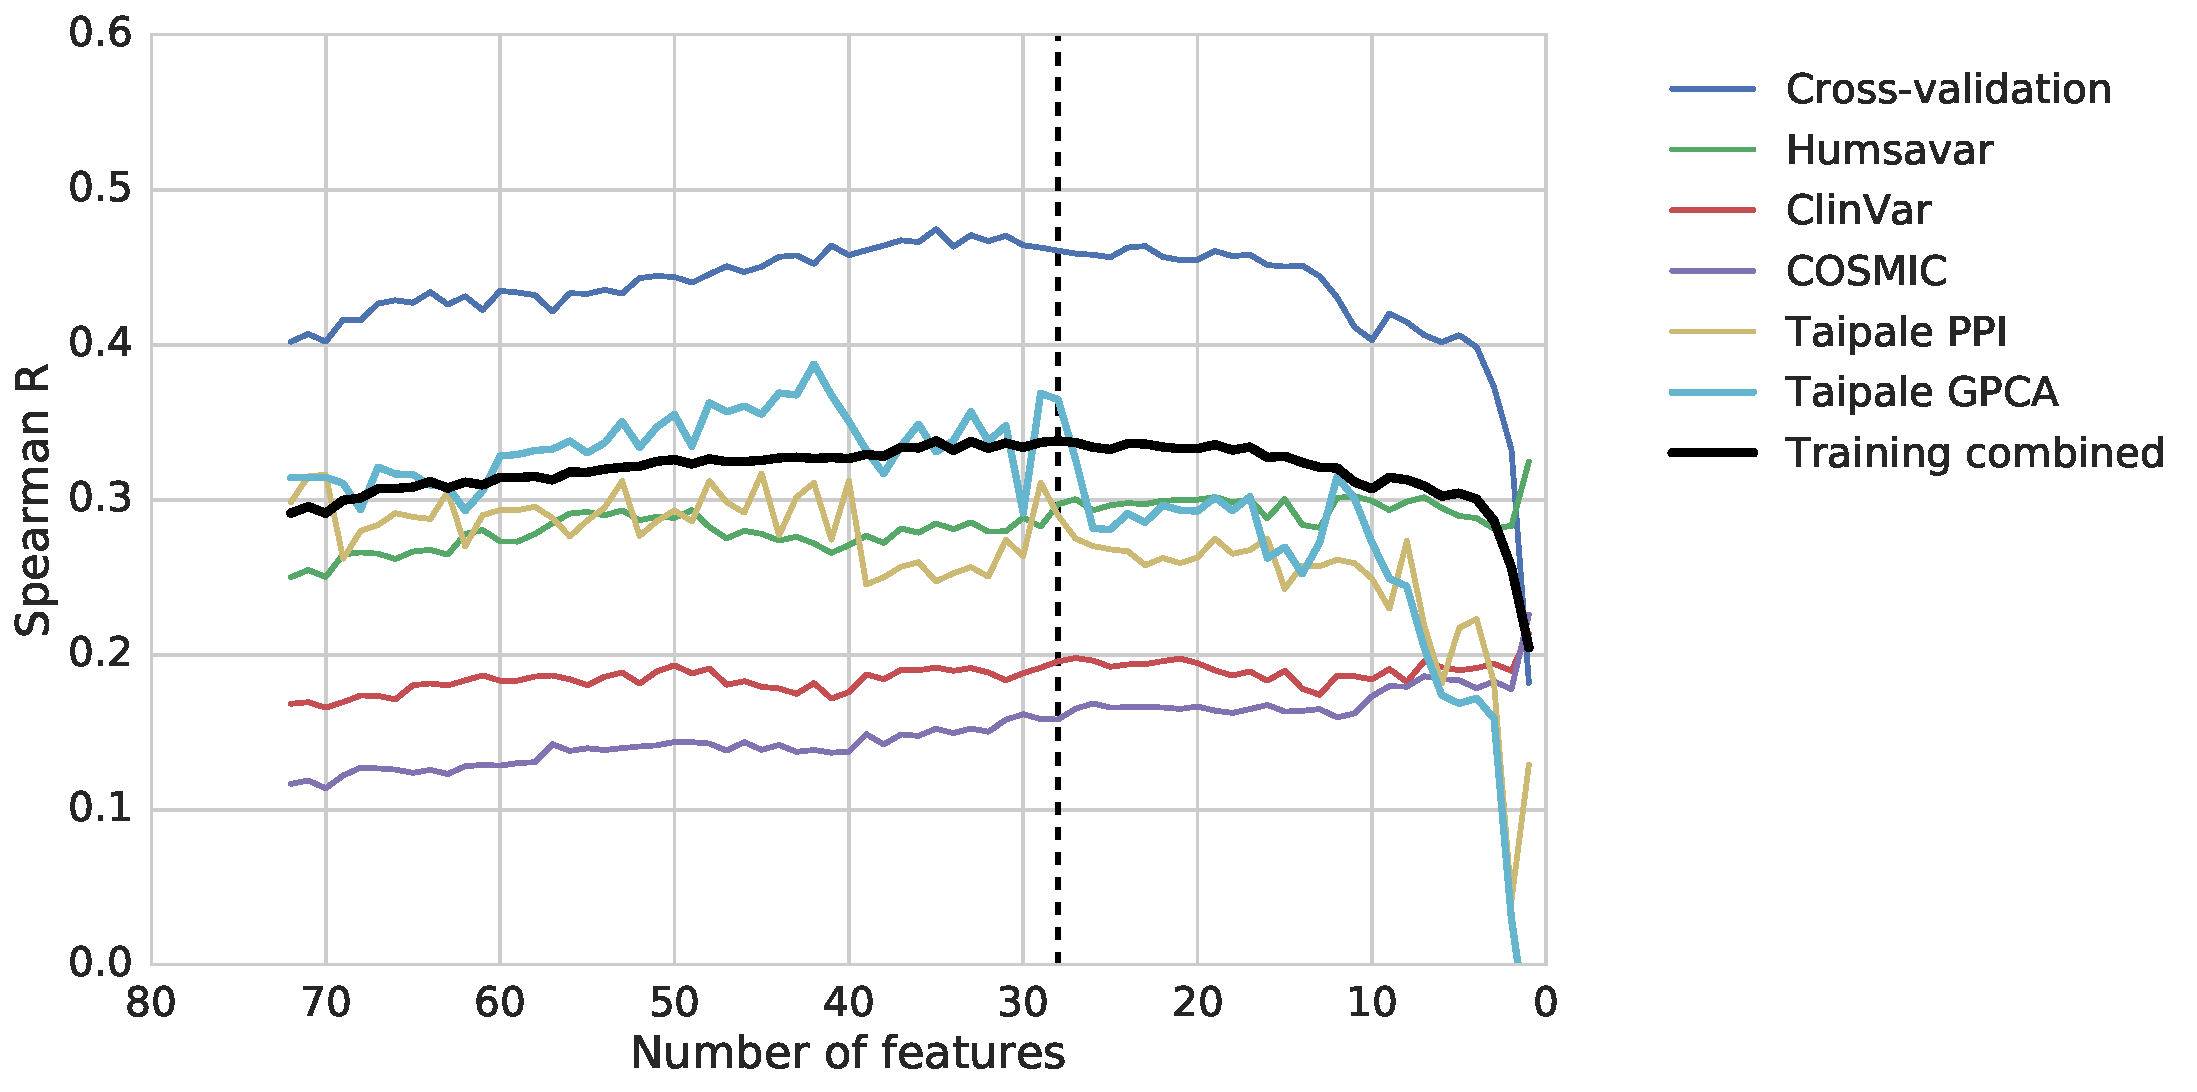
\includegraphics[width=0.9\linewidth]{static/elaspic_training_set/machine_learning/feature_elimination_interface.pdf}
	\caption[Interface predictor feature elimination.]{
		Performance of the interface predictor at each step of feature elimination.
		The combined score (black line) was calculated using Equation \ref{eq:combined_score_interface}.
		Predictor with the highest combined score is indicated by the vertical dashed line,
		and the features used to train that predictor are listed in Table \ref{tab:interface_features}.
	}
	\label{fig:feature_elimination_interface}
\end{figure}

\clearpage

\begin{table}[tb]
	\centering
	\caption[Features selected for the core predictor.]{
		Core predictor features.
		Features that end in \textit{\_wt} were computed for the wild-type structure.
		Features that end in \textit{\_change} correspond to the difference between the values computed for the wild-type and mutant structures.
		Rows in bold mark the 6 most important features.
		FoldX feature descriptions were taken from \url{http://foldxsuite.crg.eu/command/Stability}.
	}
	\label{tab:core_features}
	\begin{tabular}{ l | l | p{7cm} }
		\toprule
		Feature name                              & Feature source   & Feature description                                                                                                   \\
		\midrule
		alignment\_coverage                       & ELASPIC          & Alignment coverage.                                                                                                   \\
		alignment\_identity                       & ELASPIC          & Alignment sequence identity.                                                                                          \\
		alignment\_score                          & ELASPIC          & Alignment quality (Equation \ref{eq:core_alignment_score}).                                                           \\
		backbone\_hbond\_change                   & FoldX            & Backbone hydrogen bond energy.                                                                                        \\
		backbone\_hbond\_wt                       & FoldX            & Backbone hydrogen bond energy.                                                                                        \\
		cis\_bond\_wt                             & FoldX            & Cis peptide bond energy.                                                                                              \\
		disulfide\_wt                             & FoldX            & Disulfide bond energy.                                                                                                \\
		electrostatic\_kon\_change                & FoldX            & Electrostatic interaction between molecules in the pre-complex.                                                       \\
		\textbf{electrostatics\_change}           & \textbf{FoldX}   & \textbf{Electrostatic interactions.}                                                                                  \\
		entropy\_mainchain\_change                & FoldX            & Entropy cost of fixing the main chain.                                                                                \\
		helix\_dipole\_wt                         & FoldX            & Electrostatic contribution of the helix dipole.                                                                       \\
		matrix\_score                             & ELASPIC          & BLOSUM62 matrix score.                                                                                                \\
		pcv\_hbond\_change                        & ELASPIC          & Hydrogen-oxygen contacts involving atoms of the mutated residue and water molecules present in the crystal structure. \\
		pcv\_hbond\_self\_change                  & ELASPIC          & Hydrogen-oxygen contacts involving atoms of the mutated residue and atoms of the mutated chain.                       \\
		pcv\_salt\_equal\_change                  & ELASPIC          & Charge repulsions between atoms of the mutated residue and ions and heteroatoms present in the crystal structure.     \\
		pcv\_salt\_equal\_self\_wt                & ELASPIC          & Charge repulsions between atoms of the mutated residue and atoms of the mutated chain.                                \\
		pcv\_salt\_equal\_wt                      & ELASPIC          & Charge repulsions between atoms of the mutated residue and ions and heteroatoms present in the crystal structure      \\
		pcv\_salt\_opposite\_change               & ELASPIC          & Charge attractions between atoms of the mutated residue and ions and heteroatoms present in the crystal structure.    \\
		pcv\_vdw\_self\_change                    & ELASPIC          & Carbon carbon contacts between atoms of the mutated residue and atoms of the mutated chain.                           \\
		\textbf{provean\_score}                   & \textbf{Provean} & \textbf{Sequence conservation score.}                                                                                 \\
		sloop\_entropy\_wt                        & FoldX            & Entropic cost according to the SLoop database of loop conformations.                                                  \\
		\textbf{solvation\_hydrophobic\_change}   & \textbf{FoldX}   & \textbf{Contribution of hydrophobic groups.}                                                                          \\
		\textbf{solvation\_polar\_change}         & \textbf{FoldX}   & \textbf{Energetic penalty for burying polar groups.}                                                                  \\
		\textbf{solvent\_accessibility\_wt}       & \textbf{MSMS}    & \textbf{Solvent-accessible surface area of the mutated residue.}                                                      \\
		torsional\_clash\_change                  & FoldX            & Intra-residue van der Waals torsional clashes.                                                                        \\
		\textbf{van\_der\_waals\_clashes\_change} & \textbf{FoldX}   & \textbf{Energy penalization due to van der Waals clashes (interresidue).}                                             \\
		water\_bridge\_wt                         & FoldX            & Contribution of water bridges.                                                                                        \\
		\bottomrule
	\end{tabular}
\end{table}

\begin{table}[tb]
	\centering
	\caption[Features selected for the interface predictor.]{
		Interface predictor features.
		Features that end in \textit{\_wt} were computed for the wild-type structure.
		Features that end in \textit{\_change} correspond to the difference between the values computed for the wild-type and mutant structures.
		Rows in bold mark the 6 most important features.
		FoldX feature descriptions were taken from \url{http://foldxsuite.crg.eu/command/AnalyseComplex}.
	}
	\label{tab:interface_features}
	\begin{tabular}{ l | l | p{8cm} }
		\toprule
		Feature name                          & Feature source   & Feature description                                                                                        \\
		\midrule
		alignment\_score                      & ELASPIC          & Alignment quality (Equation \ref{eq:interface_alignment_score}).                                           \\
		backbone\_clash\_change               & FoldX            & Backbone-backbone van der Waals energy.                                                                    \\
		backbone\_clash\_wt                   & FoldX            & Backbone-backbone van der Waals energy.                                                                    \\
		backbone\_hbond\_change               & FoldX            & Backbone hydrogen bond energy.                                                                             \\
		cis\_bond\_wt                         & FoldX            & Cis peptide bond energy.                                                                                   \\
		electrostatic\_kon\_wt                & FoldX            & Electrostatic interaction between molecules in the pre-complex.                                            \\
		energy\_ionisation\_wt                & FoldX            & Ionization energy.                                                                                         \\
		entropy\_complex\_change              & FoldX            & Entropic cost of forming a complex.                                                                        \\
		\textbf{entropy\_sidechain\_change}   & \textbf{FoldX}   & \textbf{Entropic cost of fixing the side chain.}                                                           \\
		intraclashes\_energy\_2\_change       & FoldX            & van der Waals clashes of residues at the interface of the complex.                                         \\
		\textbf{partial\_covalent\_bonds\_wt} & \textbf{FoldX}   & \textbf{Interactions with bound metals.}                                                                   \\
		pcv\_hbond\_self\_change              & ELASPIC          & Hydrogen-oxygen contacts involving atoms of the mutated residue and atoms of the mutated chain.            \\
		pcv\_hbond\_wt                        & ELASPIC          & Hydrogen-oxygen contacts involving atoms of the mutated residue and atoms of the interacting chain.        \\
		pcv\_salt\_equal\_self\_change        & ELASPIC          & Charge repulsions involving atoms of the mutated residue and atoms of the mutated chain.                   \\
		pcv\_salt\_equal\_wt                  & ELASPIC          & Charge repulsions involving atoms of the mutated residue and atoms of the interacting chain.               \\
		pcv\_salt\_opposite\_change           & ELASPIC          & Charge attractions involving atoms of the mutated residue and atoms of the interacting chain.              \\
		pcv\_salt\_opposite\_self\_change     & ELASPIC          & Charge attractions involving atoms of the mutated residue and atoms of the mutated chain.                  \\
		pcv\_salt\_opposite\_self\_wt         & ELASPIC          & Charge attractions involving atoms of the mutated residue and atoms of the mutated chain.                  \\
		pcv\_vdw\_self\_change                & ELASPIC          & Carbon carbon contacts involving atoms of the mutated residue and atoms of the mutated chain.              \\
		\textbf{pcv\_vdw\_self\_wt}           & \textbf{ELASPIC} & \textbf{Carbon carbon contacts involving atoms of the mutated residue and atoms of the mutated chain.}     \\
		\textbf{pcv\_vdw\_wt}                 & \textbf{ELASPIC} & \textbf{Carbon carbon contacts involving atoms of the mutated residue and atoms of the interacting chain.} \\
		\textbf{provean\_score}               & \textbf{Provean} & \textbf{Sequence conservation score.}                                                                      \\
		sloop\_entropy\_change                & FoldX            & Entropic cost according to the SLoop database of loop conformations.                                       \\
		solvation\_hydrophobic\_change        & FoldX            & Contribution of hydrophobic groups.                                                                        \\
		\textbf{solvation\_polar\_change}     & \textbf{FoldX}   & \textbf{Energetic penalty for burying polar groups.}                                                       \\
		solvation\_polar\_wt                  & FoldX            & Energetic penalty for burying polar groups.                                                                \\
		torsional\_clash\_change              & FoldX            & Intra-residue van der Waals torsional clashes.                                                             \\
		water\_bridge\_change                 & FoldX            & Contribution of water bridges.                                                                             \\
		\bottomrule
	\end{tabular}
\end{table}
